
\clearpage
\section{Controlling}

\begin{wrapfigure}[7]{l}{6.5cm}   % [x] Wie manche Zeile soll sich um die Grafik "brechen"
  \vspace{-35pt}      % Grundwert war 20; mit 30 schön oben beim Text ausgerichtet
  \begin{center}
    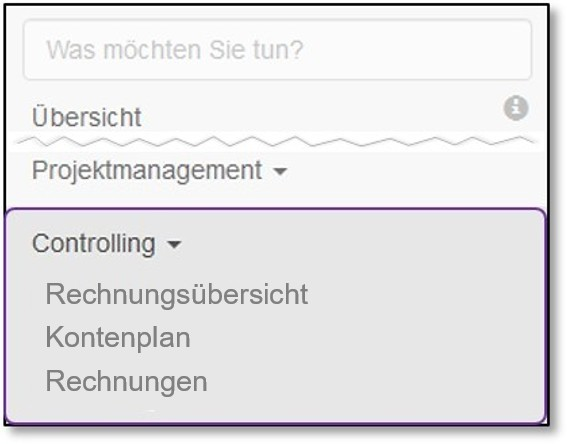
\includegraphics[width=1\linewidth]{../chapters/07_Controlling/pictures/contr_Uebersicht.jpg}
  \end{center}
  \vspace{-20pt}
  \caption{Das Controlling-Menü}
  \vspace{-10pt}
\end{wrapfigure}

Dieses Modul ermöglicht Ihnen in Anlehnung an das Beschaffungswesen eine gute Kostenübersicht über ein Projekt.
Ausgehend von Beschaffungen und Verträgen werden diese mit dem Kontenplan verknüpft. Der Kontenplan kann in eine Struktur über- und untergeordneter Abhängigkeiten von Konten erstellt werden.

\vspace{2cm} 

Wurde der Kontenplan erstellt, werden in einem zweiten Schritt sämtliche Rechnungen erfasst und einem Konto (Ausgabestelle) zugeordnet. In der Rechnungsübersicht sehen Sie tabellarisch wie hoch die Vertragsbeträge sind, die Rechnungen in Bezug auf ein Konto werden zusammengezählt und der noch verbleibende Kostenteil wird errechnet. So haben Sie stets eine praktische Übersicht über die laufenden Beschaffungs- und Projektkosten.


\subsection{Controlling-Übersicht}
\label{bkm:Ref2018080602}

\begin{figure}[H]
\center{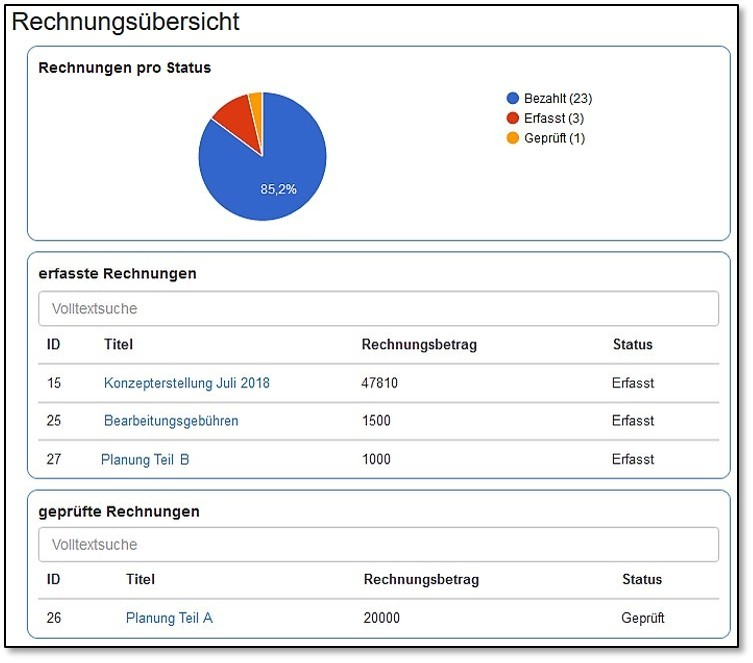
\includegraphics[width=.75\linewidth]{../chapters/07_Controlling/pictures/contr_Dashboard.jpg}}
\caption{Das Controlling Dashboard}
% \label{fig:speciation}
\end{figure}

Das Controlling Dashboard zeigt Ihnen grafisch an, wie viele Rechnungen welchen Zustand (Status) haben. In den Tabellen sind dann die Rechnungen aufgeführt, welche erfasst jedoch noch nicht geprüft und zum Zweiten geprüft, aber noch nicht freigegeben wurden. Mit Klick auf den Rechnungstitel gelangen Sie direkt in den Bearbeitungsmodus der Rechnung und können diese weiterverarbeiten, respektive den Status ändern.

\vspace{\baselineskip}

\textbf{Hinweis:} Dashboards sind kundenspezifisch konfigurierbar. Entsprechend kann die Ansicht Ihrer CUBE PA-Instanz anders aussehen als in diesem Handbuch abgebildet.

\vspace{\baselineskip}

\begin{figure}[H]
\center{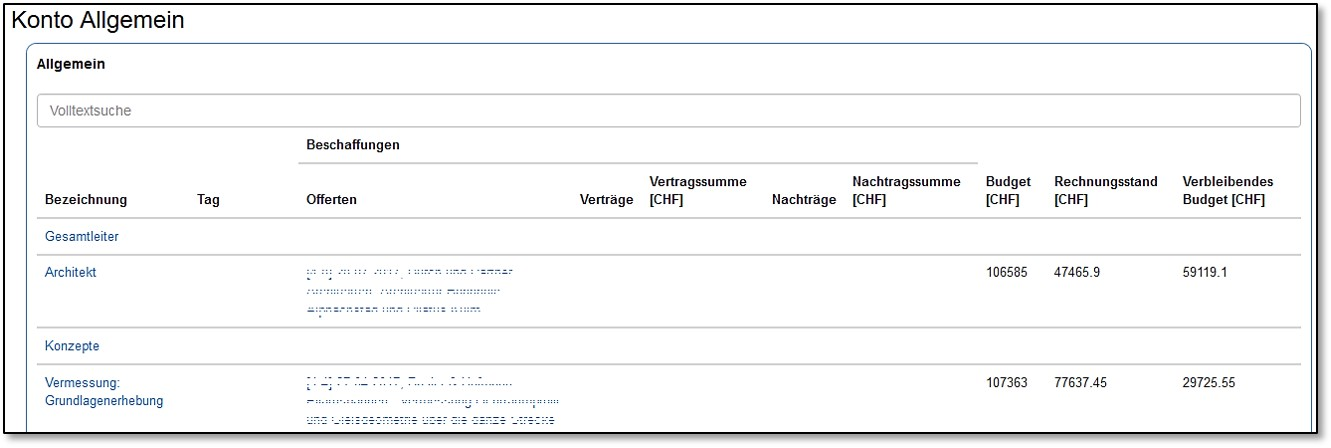
\includegraphics[width=1\linewidth]{../chapters/07_Controlling/pictures/contr_Kontouebersicht.jpg}}
\caption{Die Kontenübersicht}
% \label{fig:speciation}
\end{figure}

In der Kontenübersicht sind wie eingangs beschrieben, sämtliche Konten-Positionen aufgeführt. Mit einem Klick können Sie in die entsprechende Beschaffung und den dazugehörigen Vertrag wechseln. Wird die Dateneingabe regelmässig gepflegt, haben Sie stets eine aktuelle Übersicht über die Beschaffungs- und Projektkosten. CUBE PA weisst die Beträge aus den Verträgen aus, zählt sämtliche eingegeben Rechnungen zusammen und hebt die Differenz zu den geplanten Kosten hervor.

\pagebreak
\subsection{Kontenplan}

\textbf{Kontenplan in der Übersicht}

\begin{figure}[H]
\center{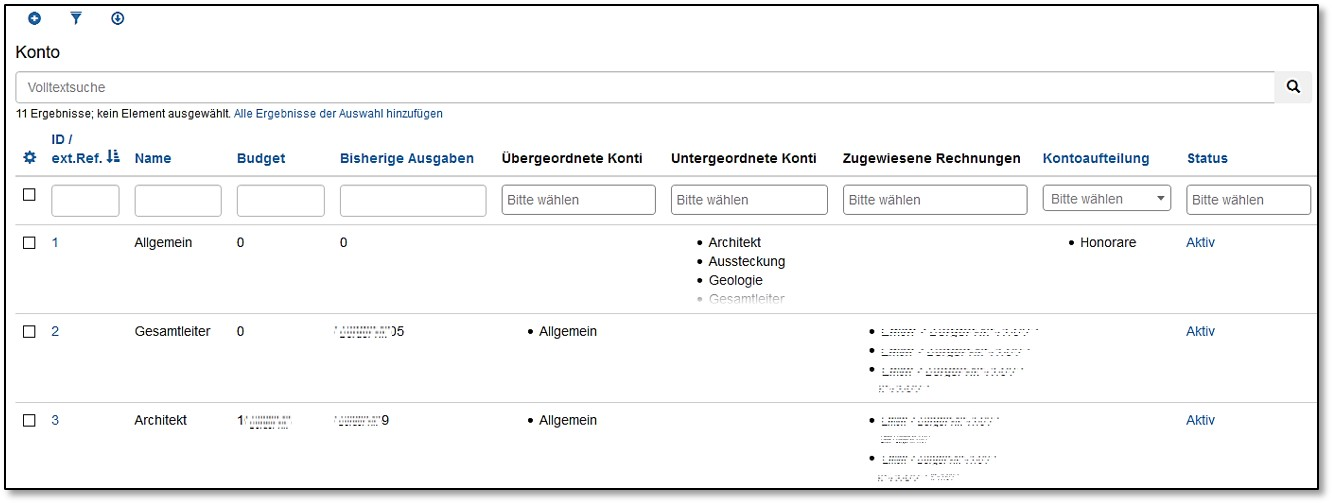
\includegraphics[width=1\linewidth]{../chapters/07_Controlling/pictures/contr_KontenplanUebersicht.jpg}}
\caption{Kontenplan in der Übersicht}
% \label{fig:speciation}
\end{figure}

Die Übersicht des Kontenplans verwendet die Standard-Funktionen des CUBE PAs. Mit dem 
\includegraphics[height=12pt]{/Icons/Plussymbol.jpg} wird ein neues Konto (Kostenstelle) hinzugefügt. Nebst der Volltextsuche oder der Filterung einzelner Spalten, können Sie weitere Filteroptionen mit dem 
\includegraphics[height=12pt]{/Icons/Filter.jpg}-Symbol einblenden.\\
Die gesuchten und gefilterten Einträge lassen sich mit dem 
\includegraphics[height=12pt]{/Icons/ListeGenerieren.jpg}-Symbol in ein Excel exportieren.

\vspace{\baselineskip}

Wollen Sie einen bestehenden Eintrag ändern oder ansehen, klicken Sie auf die blaue ID-Nummer. Die Optionen werden eingeblendet. Auch im Controlling-Modul können Sie sich eine Benachrichtigung zukommen lassen, so bald Veränderungen gemacht wurden. Mehr zu dieser Funktion in Kapitel \ref{bkm:Ref2018080601}

\vspace{\baselineskip}

\pagebreak
\textbf{Ein neues Konto erstellen:} 

\begin{figure}[H]
\center{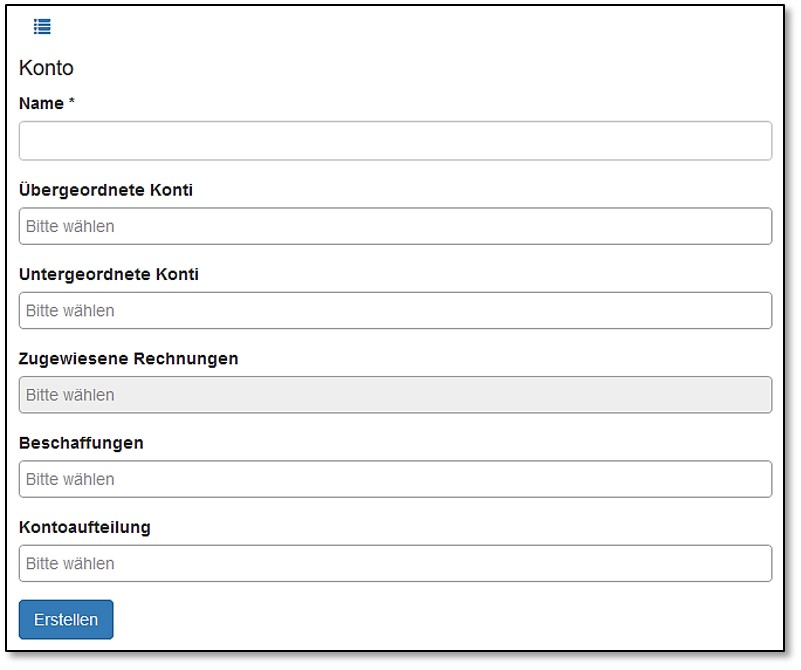
\includegraphics[width=.75\linewidth]{../chapters/07_Controlling/pictures/contr_KontoErstellen.jpg}}
\caption{Neues Konto erstellen}
% \label{fig:speciation}
\end{figure}

Geben Sie dem neuen Konto einen Namen (Pflichtfeld). Mittels den Feldern 'Übergeordnete Konti' und 'Untergeordnete Konti' können Sie innerhalb des Kontenplan eine Hierarchie / Abhängigkeit erstellen. So können Sie gewisse Kontis einer Hauptkategorie zuordnen.

\vspace{\baselineskip}

Wurden einem Konto bereits Rechnungen zugeordnet, werden diese hier auch angezeigt. Löschen oder Ändern von Rechnungen ist hier nicht möglich.\\
Weisen Sie einem Konto unbedingt eine Beschaffung zu. Nur auf diesem Weg ist es CUBE PA möglich den hinterlegten Betrag in der Beschaffung (in den Verträgen) in der Übersicht darzustellen.

\vspace{\baselineskip}

\textbf{Hinweis:} Nachträge zu einer Beschaffung werden automatisch auf der Rechnungsübersicht berücksichtigt. Achten Sie darauf, dass Sie entsprechend nur die Originalbeschaffung einem Konto zuweisen, nicht aber die Nachtragsbeschaffungen.

\vspace{\baselineskip}

Einem Konto können Sie ähnlich wie beim Dokumentenwesen Schlagworte (Tags) zuweisen. Diese werden zuvor in der Konfiguration definiert und als Kontentag markiert. Diese Definitionen übernimmt in aller Regel ein Administrator oder ein Superuser.

\pagebreak
\subsection{Rechnungen}

\textbf{Rechnungen in der Übersicht}

\begin{figure}[H]
\center{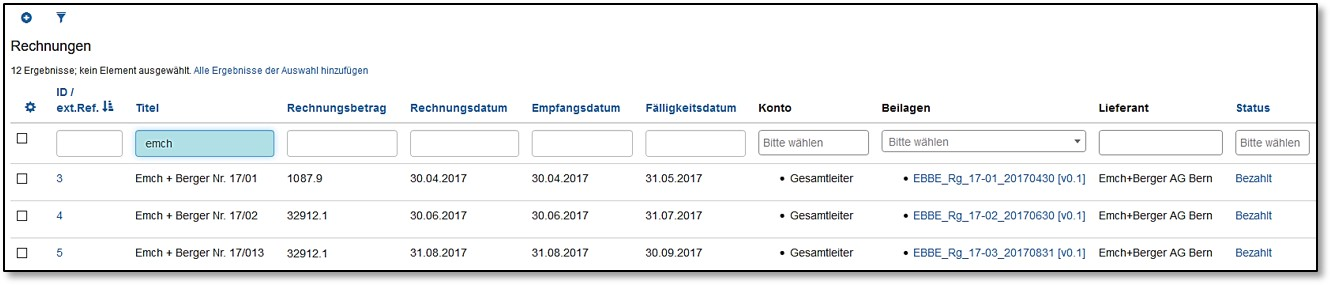
\includegraphics[width=1\linewidth]{../chapters/07_Controlling/pictures/contr_RechnungenUebersicht.jpg}}
\caption{Rechnungen in der Übersicht}
% \label{fig:speciation}
\end{figure}

In der Rechnungsübersicht befinden sich sämtliche erfassten Rechnungen. Diese können wie gewohnt nach Spalten gefiltert und sortiert werden. Mit dem Spaltenkonfigurator (
\includegraphics[height=12pt]{/Icons/SpaltenEinst.jpg}) können überflüssige Spalten zur besseren Übersicht ausgeblendet werden. Unter den Beilagen befinden sich die abgelegten Originalrechnungen (mit der Dokumentenablage verlinkt) oder sonstige Anhänge. Mit Klick darauf wechseln Sie zur entsprechneden Beilage.\\
Soll eine Rechnung bearbeitet werden, klicken Sie auf die blaue ID-Nummer. Die Optionen werden eingeblendet und Sie können das Bearbeitungssymbol (
\includegraphics[height=12pt]{/Icons/Bearbeiten.jpg}) wählen, um die nötigen Anpassungen bei einer Rechnung vorzunehmen. Wie bei den Kontis ist es auch hier möglich, sich Veränderungen an Rechnungen per Mail melden zu lassen. Mehr zum Thema Benachrichtigungen im Kapitel \ref{bkm:Ref2018080601}.

\vspace{\baselineskip}

\textbf{Vorbereitungsarbeiten für die Erfassung von Rechnungen}

\vspace{\baselineskip}

Um Rechnungen optimal erfassen zu können, empfiehlt sich, die nötigen Unteralgen (Originalrechnung, sonstige Beialgen) vorgängig zu scannen und in der Dokumentenablage bereits zu erfassen.

\vspace{\baselineskip}

\pagebreak
\textbf{Eine Rechnung erfassen}

\vspace{\baselineskip}

Wählen Sie das Plussymbol (
\includegraphics[height=12pt]{/Icons/Plussymbol.jpg}) in der Rechnungsübersicht, um einen neue Rechnung zu erfassen. Die Eingabemaske erscheint:

\begin{figure}[H]
\center{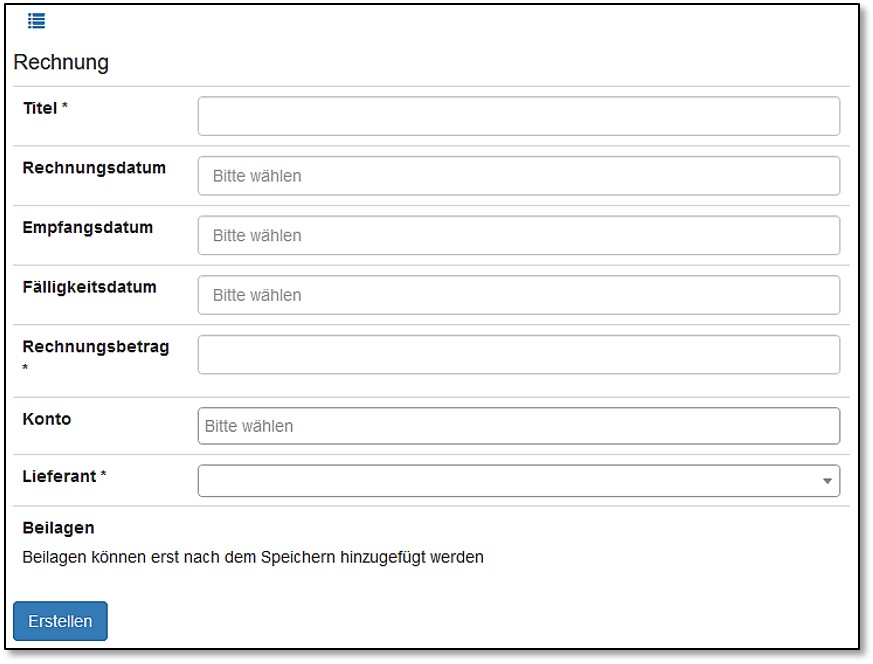
\includegraphics[width=.75\linewidth]{../chapters/07_Controlling/pictures/contr_RechnungErfassen.jpg}}
\caption{Eine Rechnung erfassen}
% \label{fig:speciation}
\end{figure}

Geben Sie einen geeigneten Titel und den Rechnungsbetrag ein (Beides sind Pflichtfelder). Weiter können Sie das Rechnungsdatum, Empfangsdatum der Rechnung, sowie das Fälligkeitsdatum hinterlegen. \\
Im nächsten Schritt wählen Sie das zugehörige Konto aus und wählen Sie den entsprechenden Lieferanten (Pflichtfeld).

\vspace{\baselineskip}

\textbf{Hinweis:} Ein Lieferant muss vorgängig erfasst werden, damit er hier in der Auswahl zur Verfügung steht.

\vspace{\baselineskip}

Nach dem erstmaligen Speichern der Daten (mittels 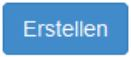
\includegraphics[height=12pt]{/Icons/B_Erstellen.jpg}) können Sie Beilagen hinzufügen. Sie können entweder Dokumente neu hochladen oder bestehende Dokumente aus der Dokumentenablage verknüpfen. Um die Beilagen zu speichern, klicken Sie erneut auf den 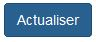
\includegraphics[height=12pt]{/Icons/B_Uebernehmen.jpg}-Button. 

\vspace{\baselineskip}

\pagebreak
\textbf{Status ändern}

\vspace{\baselineskip}

Oben im Fenster sehen Sie das Statussymbol (
\includegraphics[height=12pt]{/Icons/Status_aendern.jpg}). Eine neu erfasste Rechnung besitzt den Startstatus 'erfasst'. Klicken Sie auf das Statussymbol, um den Status zu ändern. Dieses Statussystem kann kundenspezifisch angepasst werden. Ein möglicher Statusablauf ist der folgende:

\begin{figure}[H]
\center{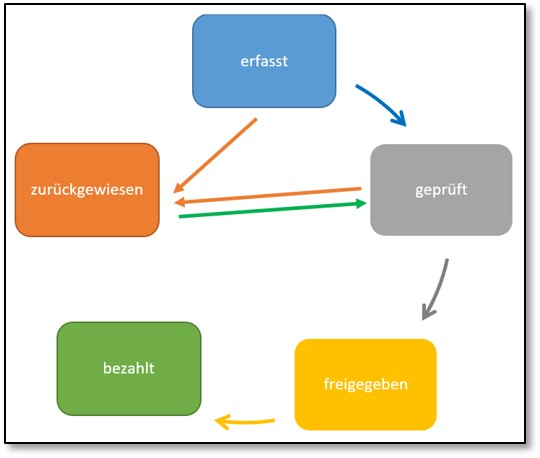
\includegraphics[width=.5\linewidth]{../chapters/07_Controlling/pictures/contr_Statussystem.jpg}}
\caption{Beispiel Statussystem}
% \label{fig:speciation}
\end{figure}
In obigem Beispiel ist es vom Status 'erfasst' und 'geprüft' möglich, eine Rechnung zurückzuweisen, da beispielsweise die Rechnung nicht korrekt oder unvollständig ist. Anschliessend kann die Rechnung vom Status 'zurückgewiesen' wieder nach 'geprüft' geändert werden.

\vspace{\baselineskip}

Im Dashboard (Kapitel \ref{bkm:Ref2018080602}) ist nun ersichtlich, wie viele Rechnungen welchen Status besitzen. In den Tabellen werden diese Rechnungen aufgelistet und mit einem Klick gelangen Sie in die gewünschte Rechnung, um sie weiter zu bearbeiten.

\vspace{\baselineskip}

Haben Sie eine weitere Rechnung erfasst, wird diese in der Kontenübersicht am entsprechenden Ort (eingetragenes Konto) aufaddiert.
